% !TEX root = cha-approach.tex
\documentclass[../../main.tex]{subfiles}

\begin{document}

\section{Path Generation via WFC}
\label{sec:path_generation_via_WFC}

In this section, we describe how we adapted and tuned the Wave Function Collapse algorithm to generate paths between classes.

\subsection{Observation Phase}
\label{subsec:wassis_observation_phase}

The observation phase consists of two steps: selecting the next cell to collapse and collapsing that cell into a tile. While standard WFC usually selects the cell with the minimum entropy, in our approach we select the cell with the \emph{maximum entropy}. Although this choice may seem counterintuitive, it is motivated by the way tile weights are defined in our tileset and by our goal: generating the paths before filling the grid with empty tiles. Empty tiles could otherwise occupy cells that may be needed by paths during generation, as shown in \figref{fig:heap_comparison}.

\begin{figure}[ht]
    \centering
    \begin{subfigure}[b]{0.48\linewidth}
        \centering
        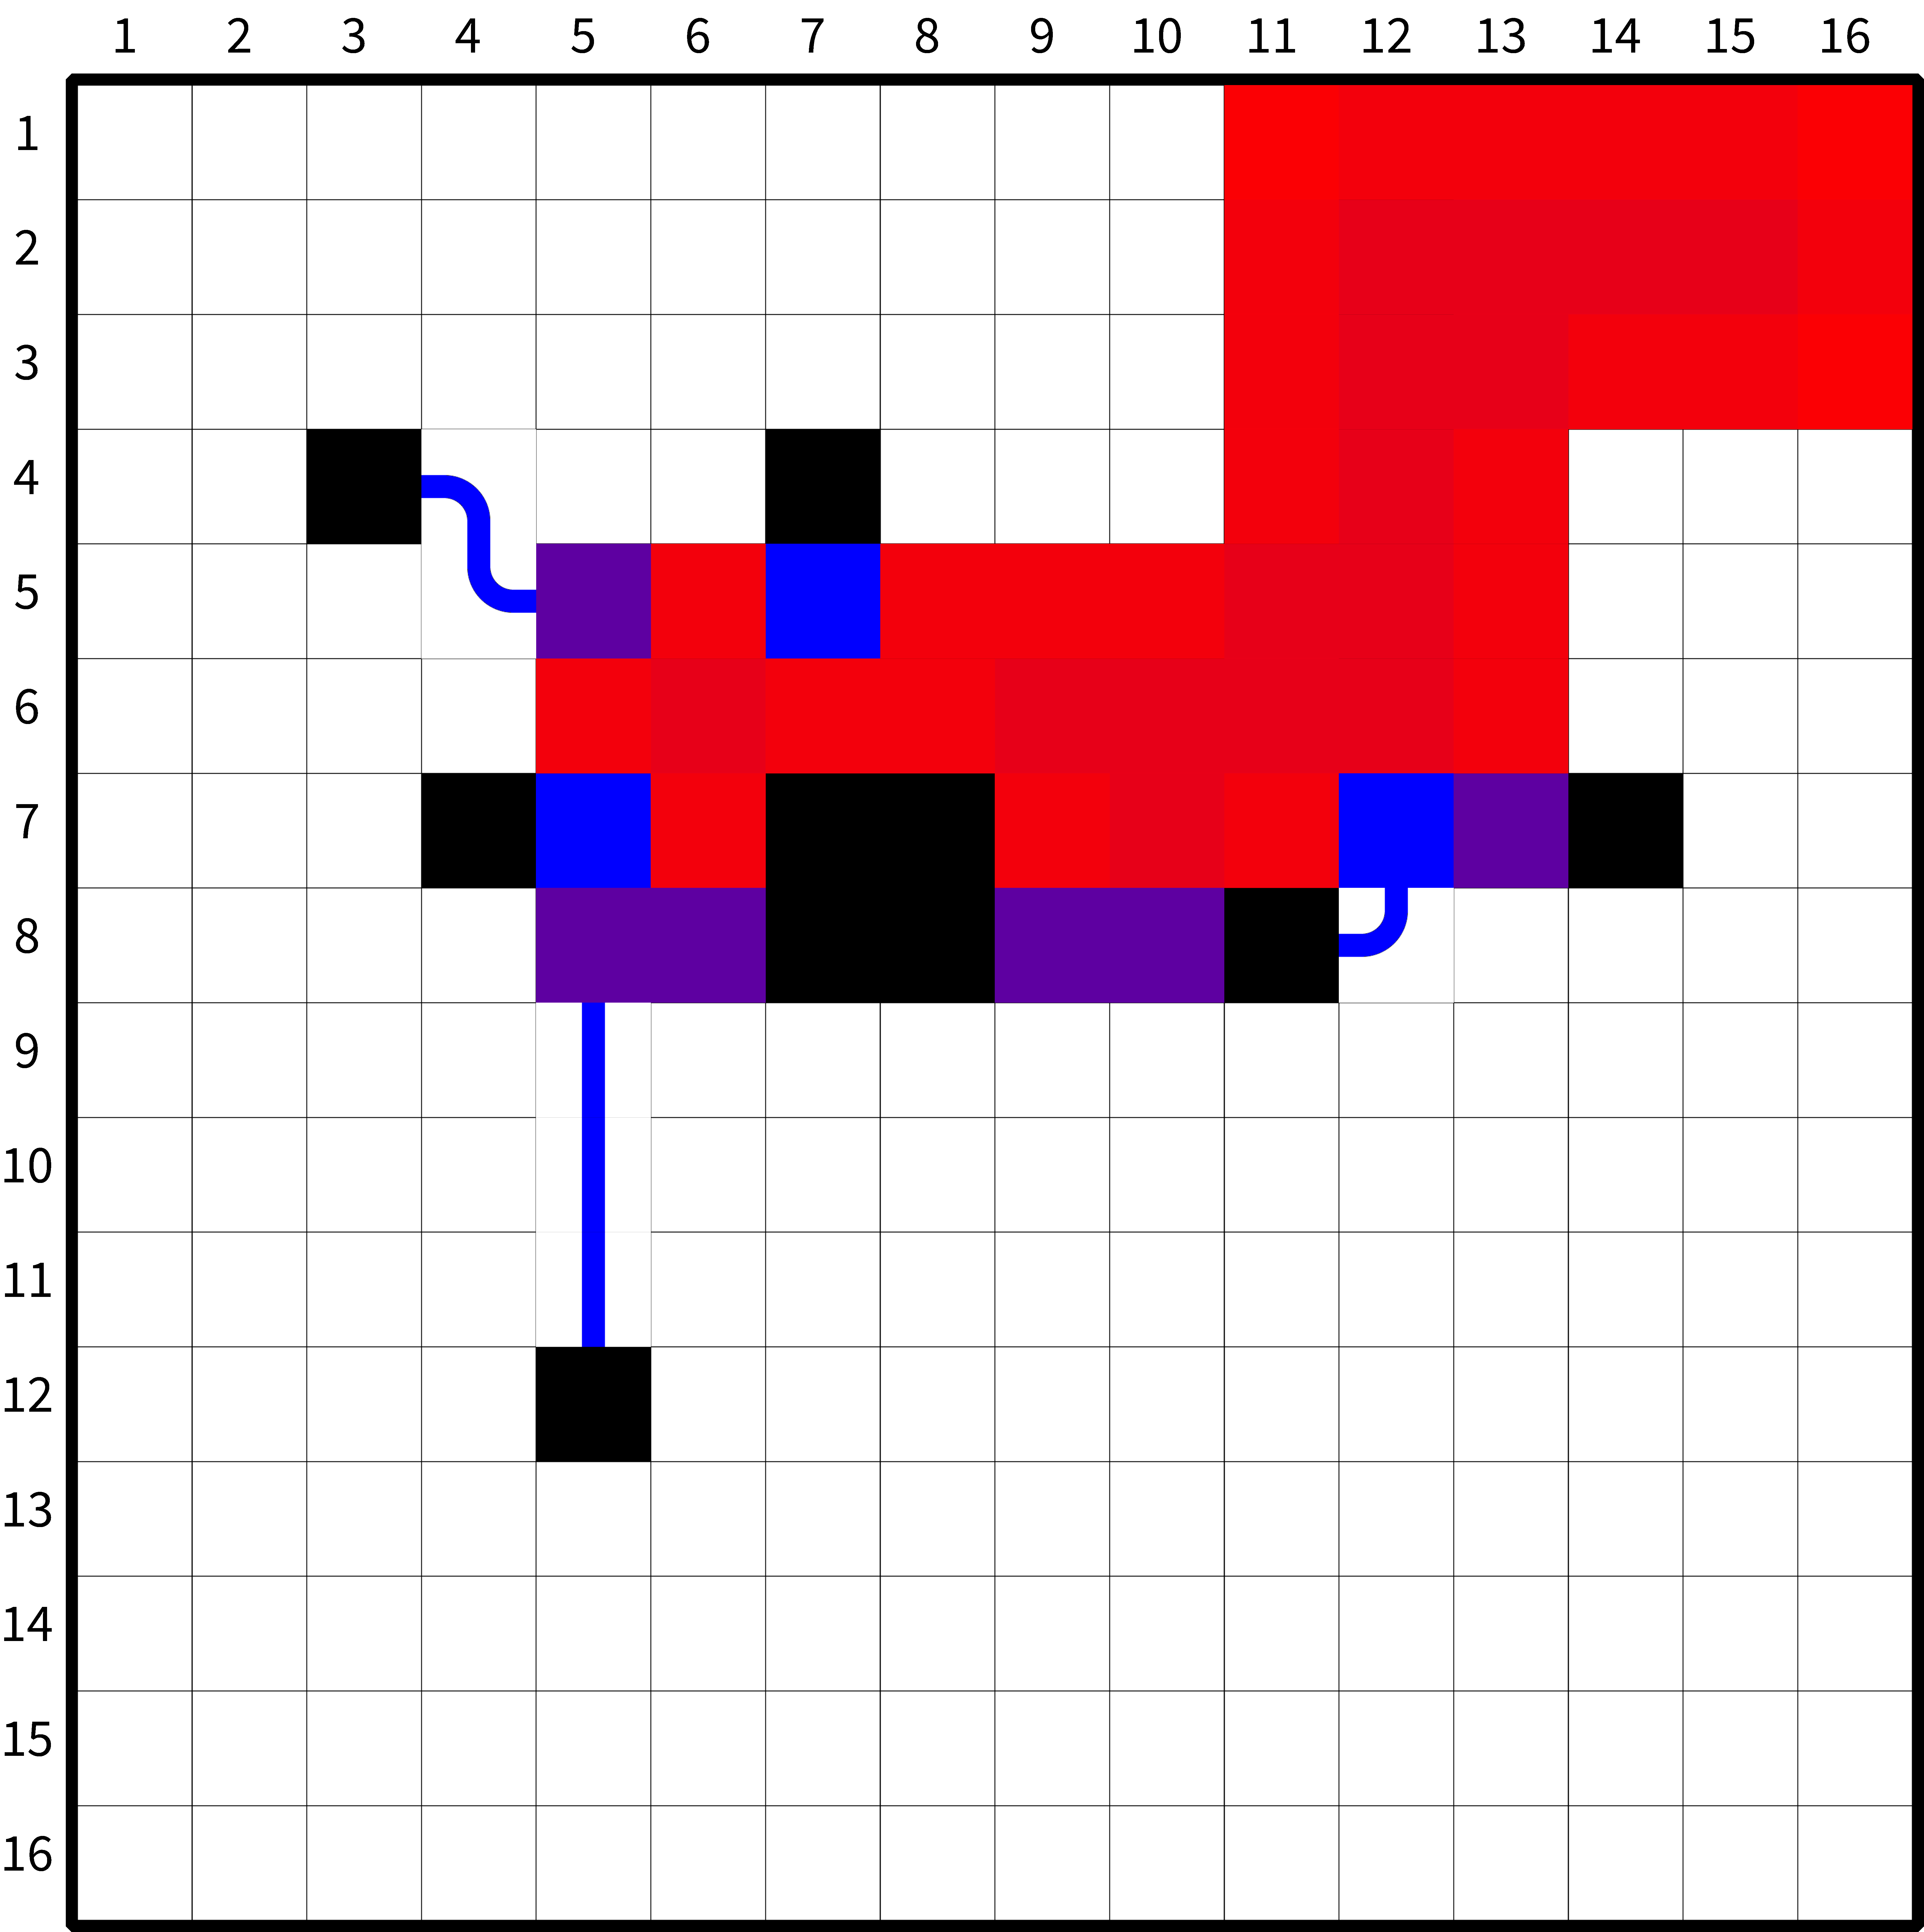
\includegraphics[width=\linewidth]{figures/approach/minHeap}
        \caption{Standard WFC using a min-heap.}
        \label{fig:min_heap}
    \end{subfigure}
    \hfill
    \begin{subfigure}[b]{0.48\linewidth}
        \centering
        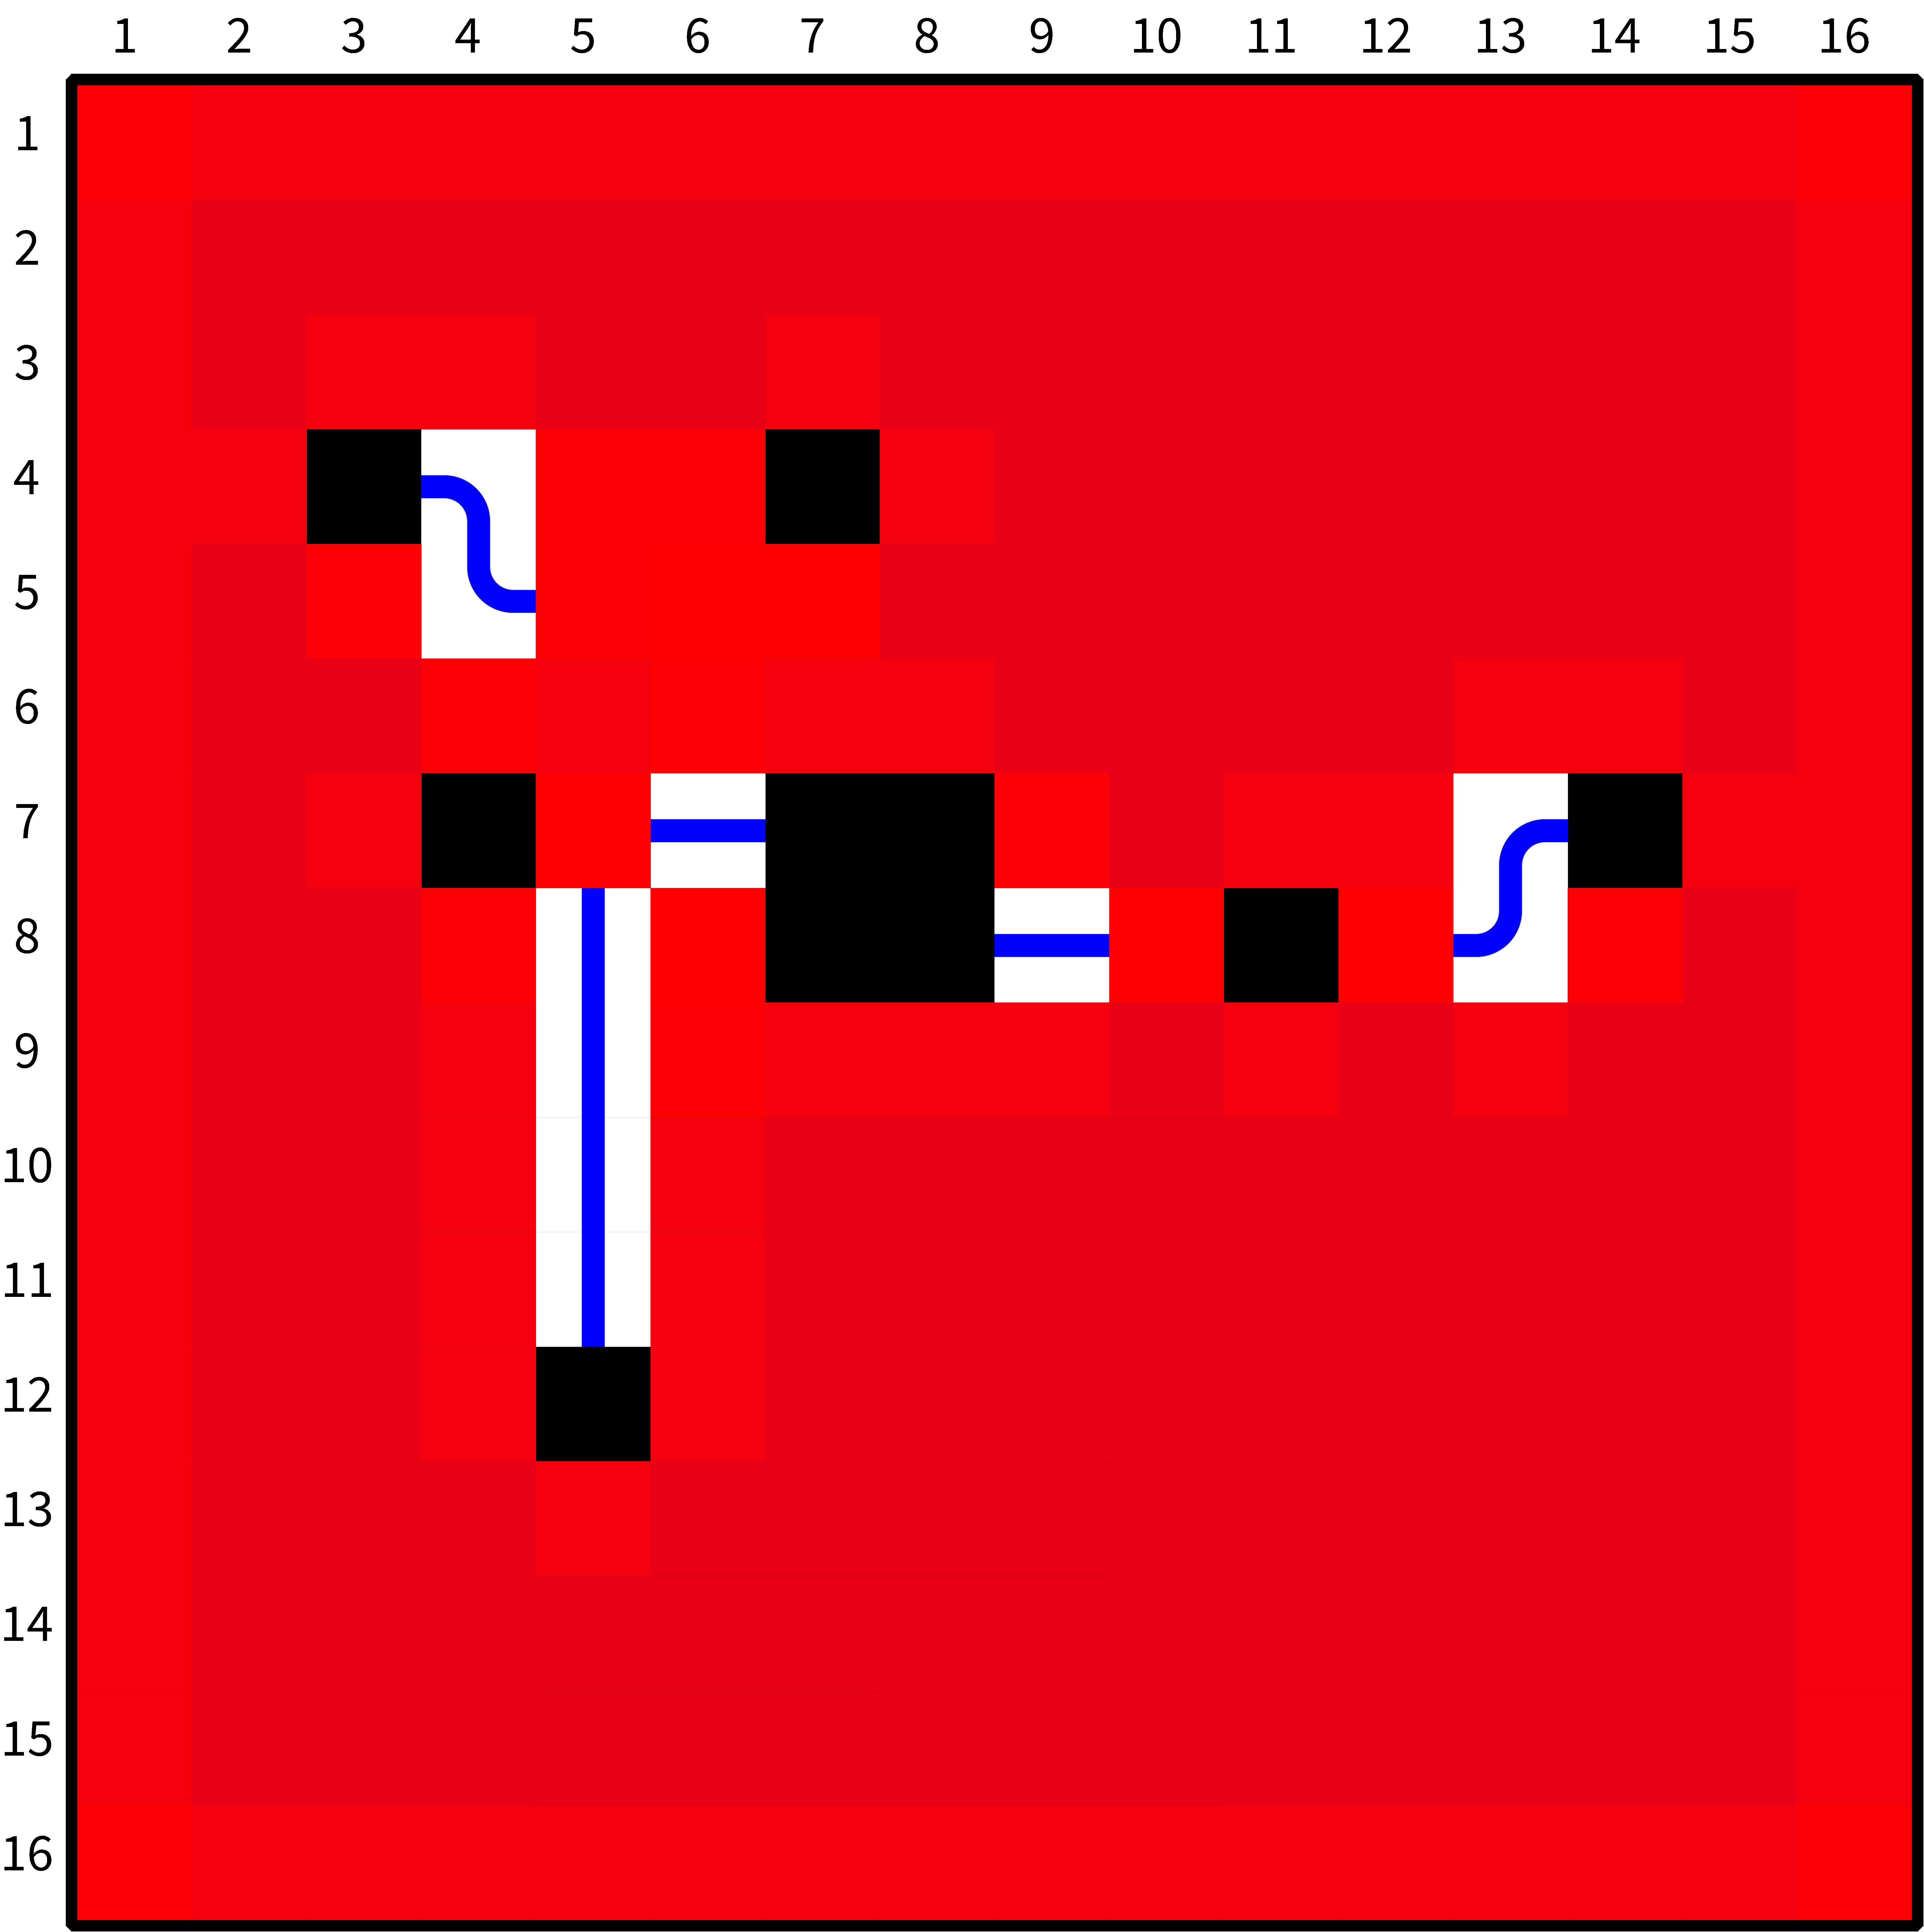
\includegraphics[width=\linewidth]{figures/approach/maxHeap}
        \caption{Our approach using a max-heap.}
        \label{fig:max_heap}
    \end{subfigure}
    \caption{Comparison of min-heap and max-heap collapse order.}
    \label{fig:heap_comparison}
\end{figure}

For the second step of the observation phase, we use a weighted random choice to select a tile from the possible tiles of the selected cell. The weights assigned to the tiles are fixed. Therefore, the entropy of a cell can be computed as:

\begin{equation}
    H = \ln \left( \sum_{i=1}^{n} w_i \right) - \frac{\sum_{i=1}^{n} w_i \ln w_i}{\sum_{i=1}^{n} w_i}
    \label{eq:shannon_entropy_unnormalized}
\end{equation}

where $w_1,\ldots,w_n$ are the weights of the possible tiles of the cell.

\noindent Note that Equation~\ref{eq:shannon_entropy_unnormalized} is the standard Shannon entropy expressed directly in terms of the tile weights instead of normalized probabilities. Proof of the equivalence with the standard formulation is shown in Appendix~\ref{sec:appendix_entropy}.

\paragraph{Tile Weights}
The weights assigned to the tiles affect both the random tile selection and the entropy used to select the next cell. The empty tile has a very large weight, while the basic path tiles, such as straight and corner tiles, have much smaller and relatively similar weights. This leads to two situations:

\begin{itemize}
    \item If the empty tile is still among the possible tiles of a cell, its large weight makes it very likely to be selected. The cell therefore has low entropy.
    \item If the empty tile has been removed by constraint propagation, only path tiles remain. Since their weights are relatively similar, the choice is less predictable and the cell has higher entropy.
\end{itemize}

\paragraph{Avoiding Unnecessary Paths}
More complex path tiles, such as T junctions, crossings, merged paths, and double paths, are assigned a weight of zero. This means they are not selected during random tile selection as long as a positive weight alternative is available. They are only used when the constraints leave no other option.

This strategy helps prevent unnecessary paths. For example, selecting a T junction when no branching is needed would create an extra branch that WFC would later have to close, potentially creating redundant loops. The same applies to crossings and other complex path tiles, which should only be used when required by the relationships being represented.

Straight and corner tiles, however, cannot have a weight of zero because they are needed to connect classes. Their weights remain much smaller than the weight of the empty tile. Therefore, when both empty and path tiles are possible, the empty tile is much more likely to be selected. This reduces the chance of generating paths in cells where they are not needed. An example of unnecessary paths is shown in \figref{fig:useless_paths}.

\begin{figure}[ht]
    \centering
    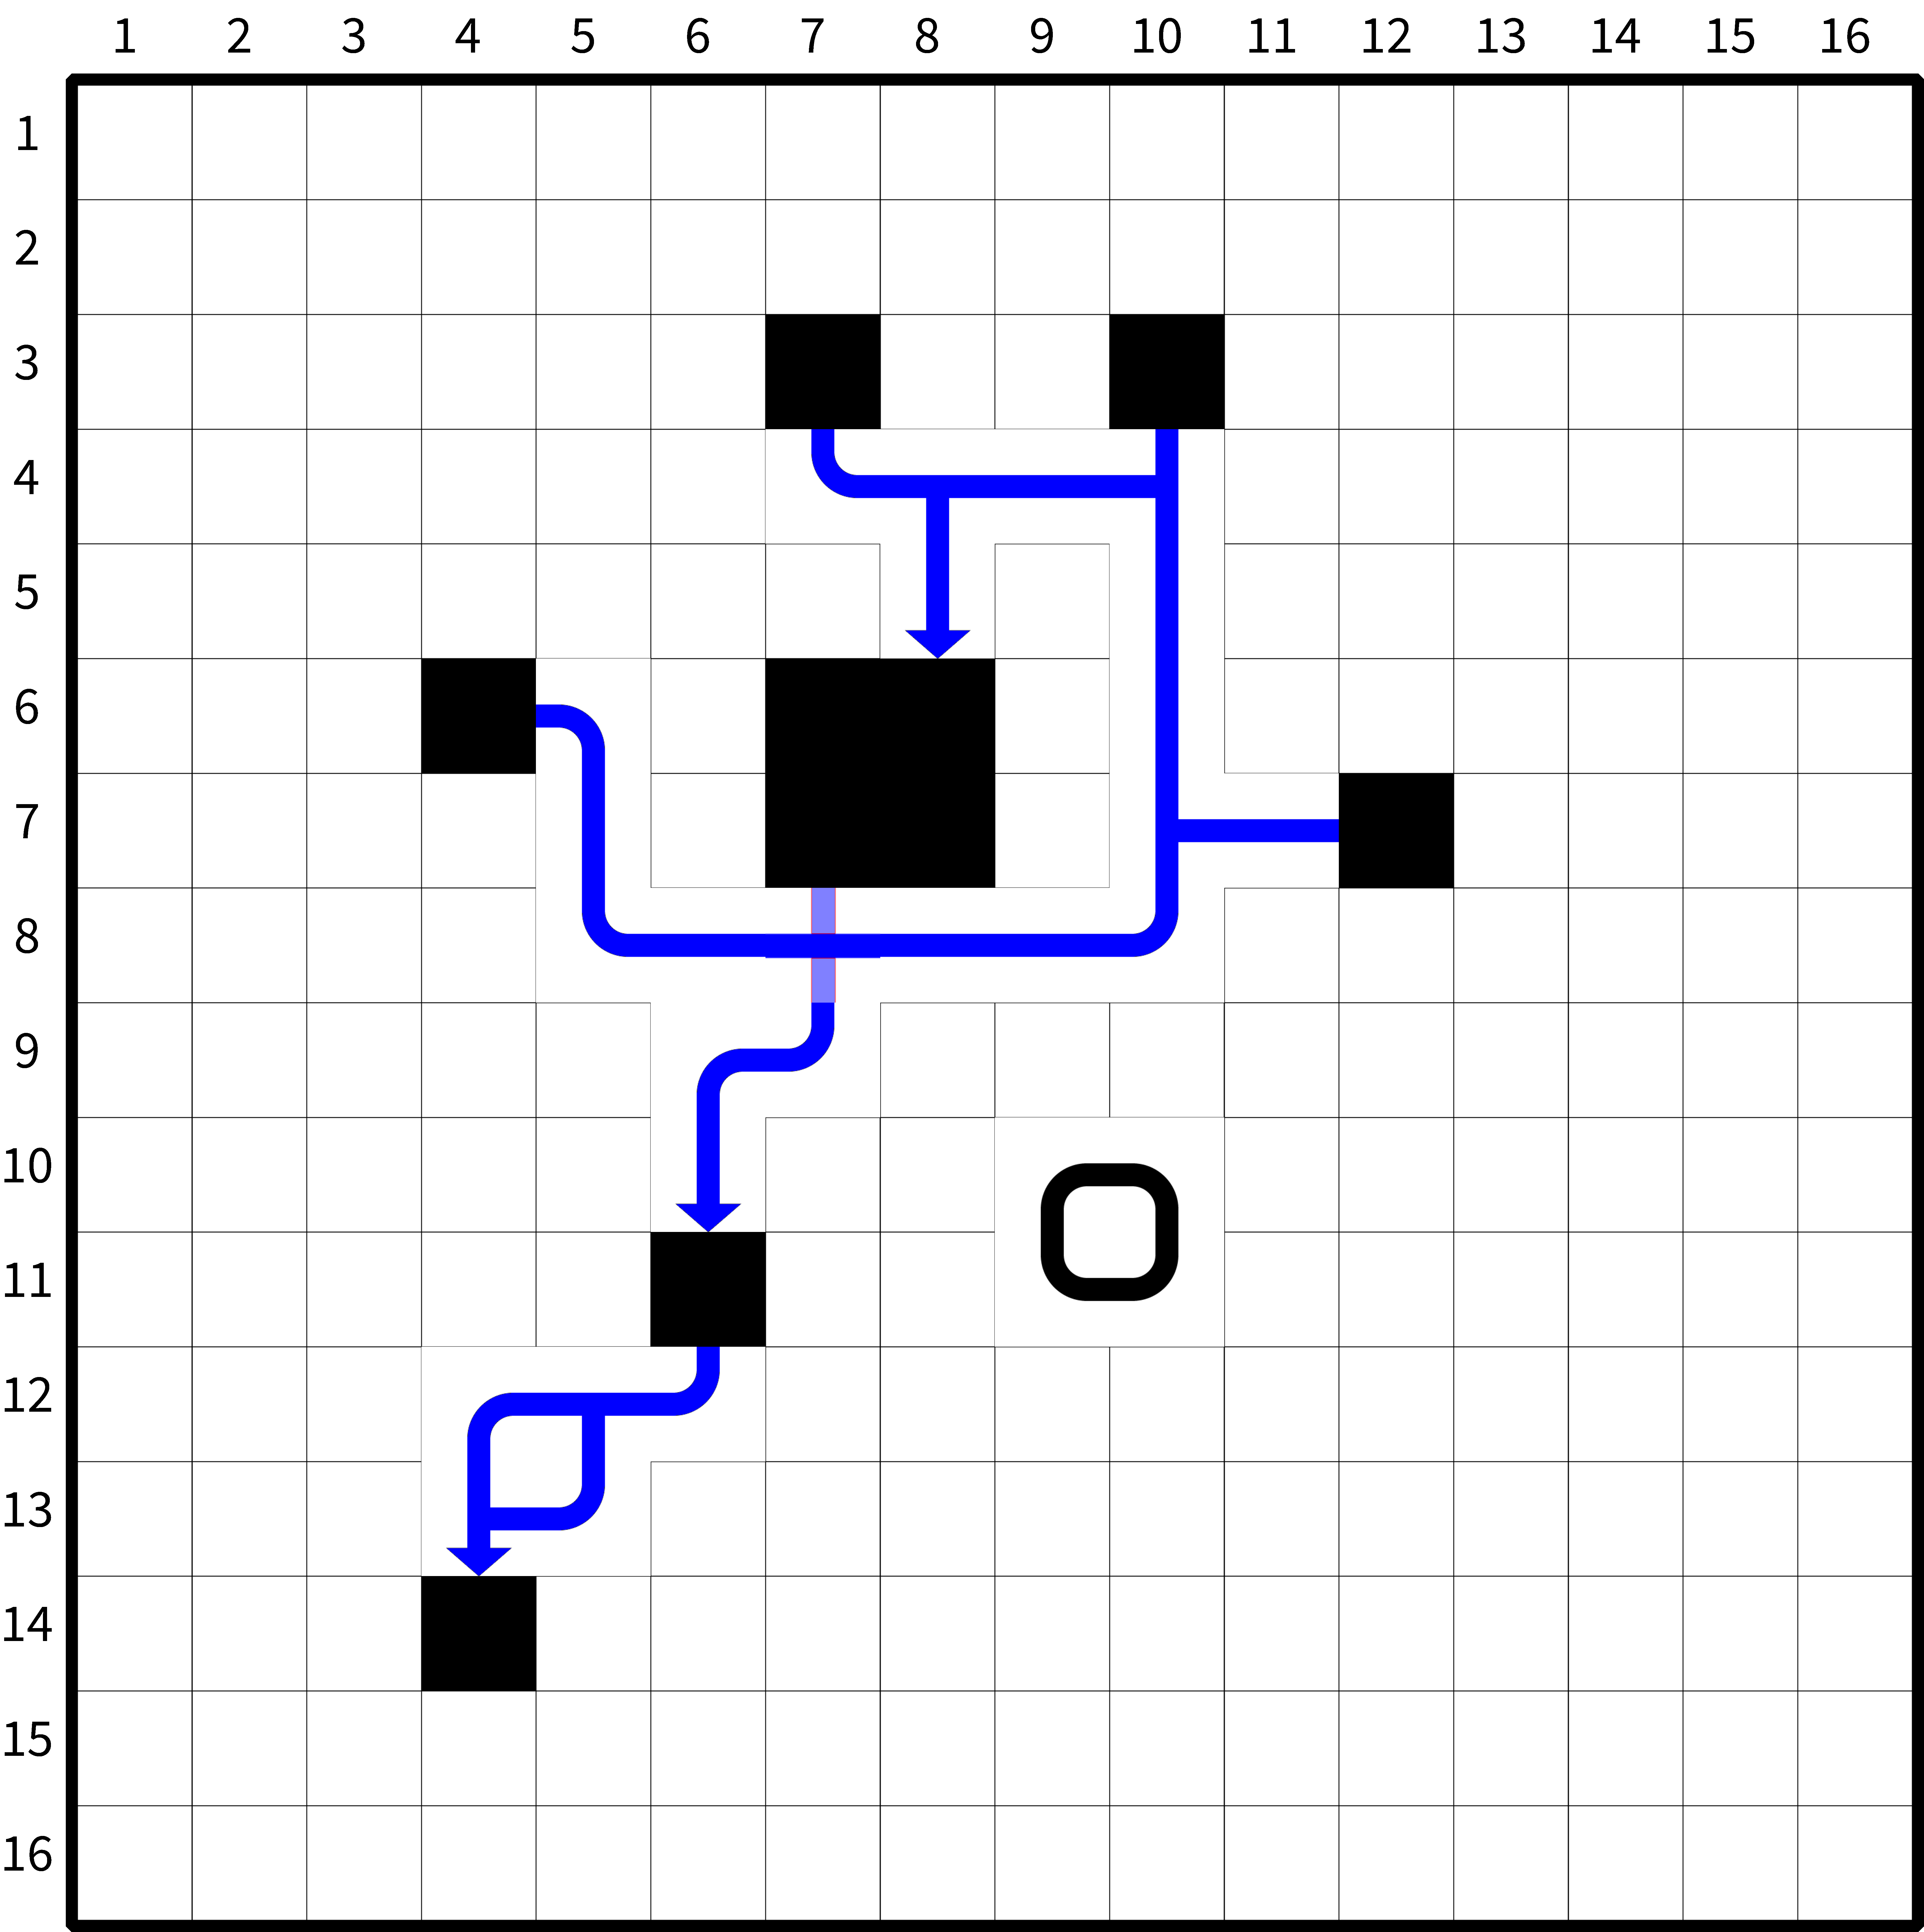
\includegraphics[width=0.6\linewidth]{figures/approach/useless_paths}
    \caption{Example of unnecessary paths generated by WFC.}
    \label{fig:useless_paths}
\end{figure}

\paragraph{Path First Generation}
The tile weights also affect the order in which cells are selected. When classes are placed on the grid, their path entry and exit points are already fixed. Constraint propagation removes the empty tile from the cells next to these points, leaving only path tiles. These cells therefore have higher entropy than cells where the empty tile is still possible. As a result, they are selected first when using maximum entropy observation. An example is shown in \figref{fig:initial_class_placement}.

As paths extend, constraint propagation removes the empty tile from neighboring cells along the paths. These cells also gain higher entropy and become candidates for the next observation. This encourages WFC to extend paths from their entry and exit points before filling the remaining grid with empty tiles.

\begin{figure}[ht]
    \centering
    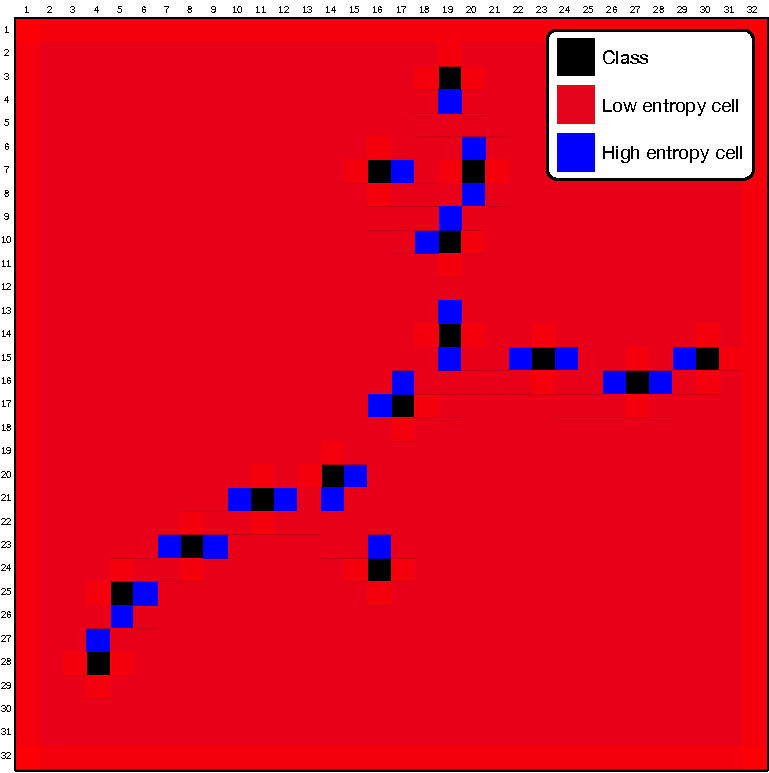
\includegraphics[width=0.6\linewidth]{figures/approach/initial_class_placement}
    \caption{Initial class placement on the grid, with fixed path entry and exit points.}
    \label{fig:initial_class_placement}
\end{figure}

Another consequence of maximum entropy observation is that paths do not necessarily close as soon as they reach their targets. Constraint propagation may leave the last cell of a path with only one possible tile or with only tiles that have a weight of zero. In both cases, the cell has low entropy and receives lower priority than cells with higher entropy.

As a result, paths can remain open while WFC generates other paths. Even after all paths have reached their targets, some final tiles may still be unassigned. WFC can therefore fill the remaining cells with empty tiles before closing these paths, as shown in \figref{fig:not_closed_paths}.

\begin{figure}
    \centering
    \includegraphics[width=0.6\linewidth]{figures/approach/not_closed_paths}
    \caption{Multiple paths remaining open during the WFC generation process.}
    \label{fig:not_closed_paths}
\end{figure}

\subsection{Propagation Phase}
After a cell is collapsed to a tile during observation, WFC propagates this choice across the grid to satisfy the local constraints.

Adjacency rules are defined using symbols assigned to each edge of a tile. Two tiles can be placed next to each other only if their touching edges have matching symbols.

When a cell loses tile options, this change is propagated to its neighbors through a loop:

\begin{enumerate}
    \item When a cell $C$ loses at least one tile option, it is added to a queue.
    \item While the queue is not empty, cell $C$ is removed from the queue, and its neighbors $N$ are checked.
    \item For each neighbor $N$, WFC removes any tile option whose symbol no longer matches at least one remaining tile in $C$.
    \item If any tile is removed from $N$, $N$ is added to the queue to update its own neighbors.
\end{enumerate}

This loop runs until the queue is empty, ensuring the grid stays consistent before the next cell is observed.

An example of complete execution of WFC is provided in \figref{fig:example_animation}.

\begin{figure}[ht]
   \centering 
   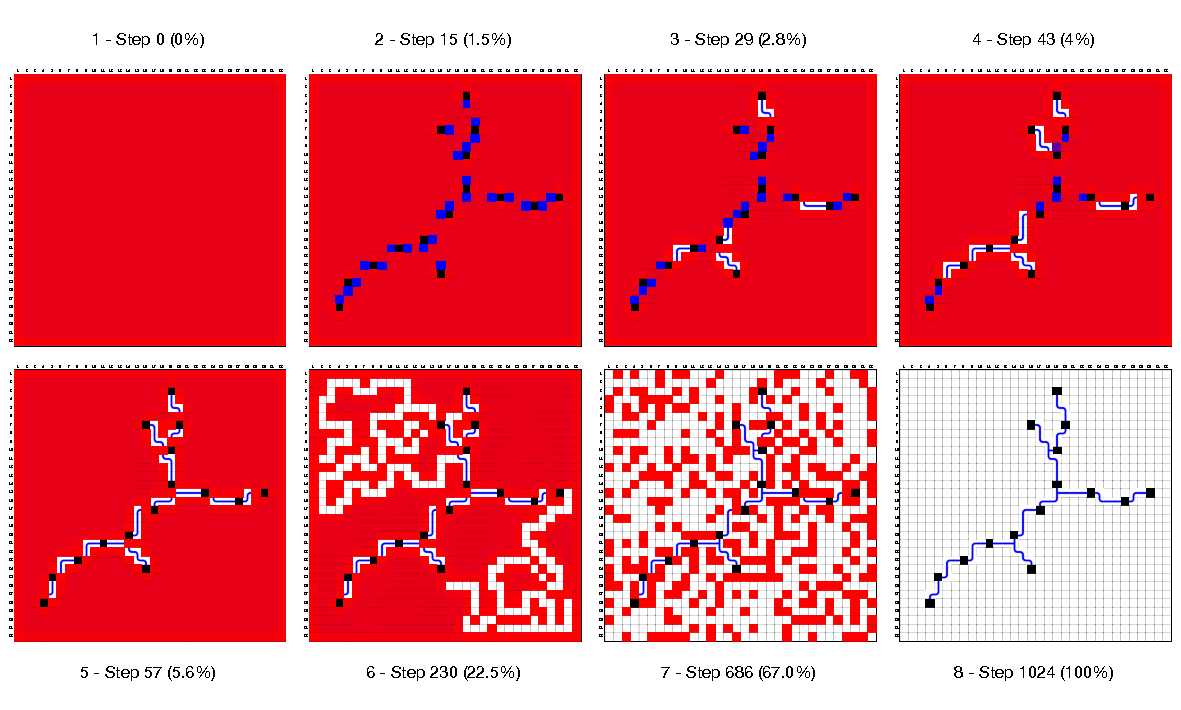
\includegraphics[width=\linewidth]{figures/approach/example_animation} 
   \caption{Animation of the execution of WFC.}
 \label{fig:example_animation}
\end{figure}

To improve the final visualization, an arrow is added to the last tile of each path to indicate its direction. This makes the direction of the relationship easier to understand, as shown in \figref{fig:final_visualization}.

\begin{figure}[ht]
   \centering 
   \includegraphics[width=0.6\linewidth]{figures/approach/final_visualization} 
   \caption{Visualization after WFC execution.}
   \label{fig:final_visualization}
\end{figure}

\end{document}